\chapter{Model Specification}
\label{chap:1} 
In this chapter we describe the abstract models used to shape all the three parts of the system.
\section{Turret Model}
Degree of Freedom (DoF) is the number of independent parameters that define the configuration of a mechanical system. In our case, we wanted to build a two DoF "Pan \& Tilt" turret. That means that our parameters are two angles. In a 3D reference system, \textbf{pan} is the horizontal angle about the upright Z axis, \textbf{tilt} is the vertical angle about the rotated Y axis. FIGURA PER MOSTRARE PAN AND TILT
Our final goal is to be able to define the direction of a laser ray mounted on top of the turret, so that we can control the position of the projected laser dot on a given surface, by solving the system's inverse kinematics.\\

For those purposes, we have built two different turrets. Since the model of the first one is slightly simpler than the second, we will start describing the former, which turns out to be helpful to understand the latter. We will focus on the case in which the laser must be projected on the ground.

\subsection{First Model}
First, figure \ref{fig:firstModel} helps us understand how we have shaped the model to match the physical structure of the turret. We have three reference frames. The \textbf{base\_link} is fixed and is the one in which we define the coordinates of the projected point. \textbf{pan\_link} and \textbf{tilt\_link} are the frames used to represent our revolute joints.
\textbf{H} is the height of the turret, which is known. Note that the convention used for the frame is the following:
\begin{itemize}
    \item red is the x axis;
    \item green is the y axis;
    \item blue is the z axis.
\end{itemize}
Thus, we consider the laser ray to be a prolongation of the x axis of the \textbf{tilt\_link}.
\begin{figure}
	\centering
	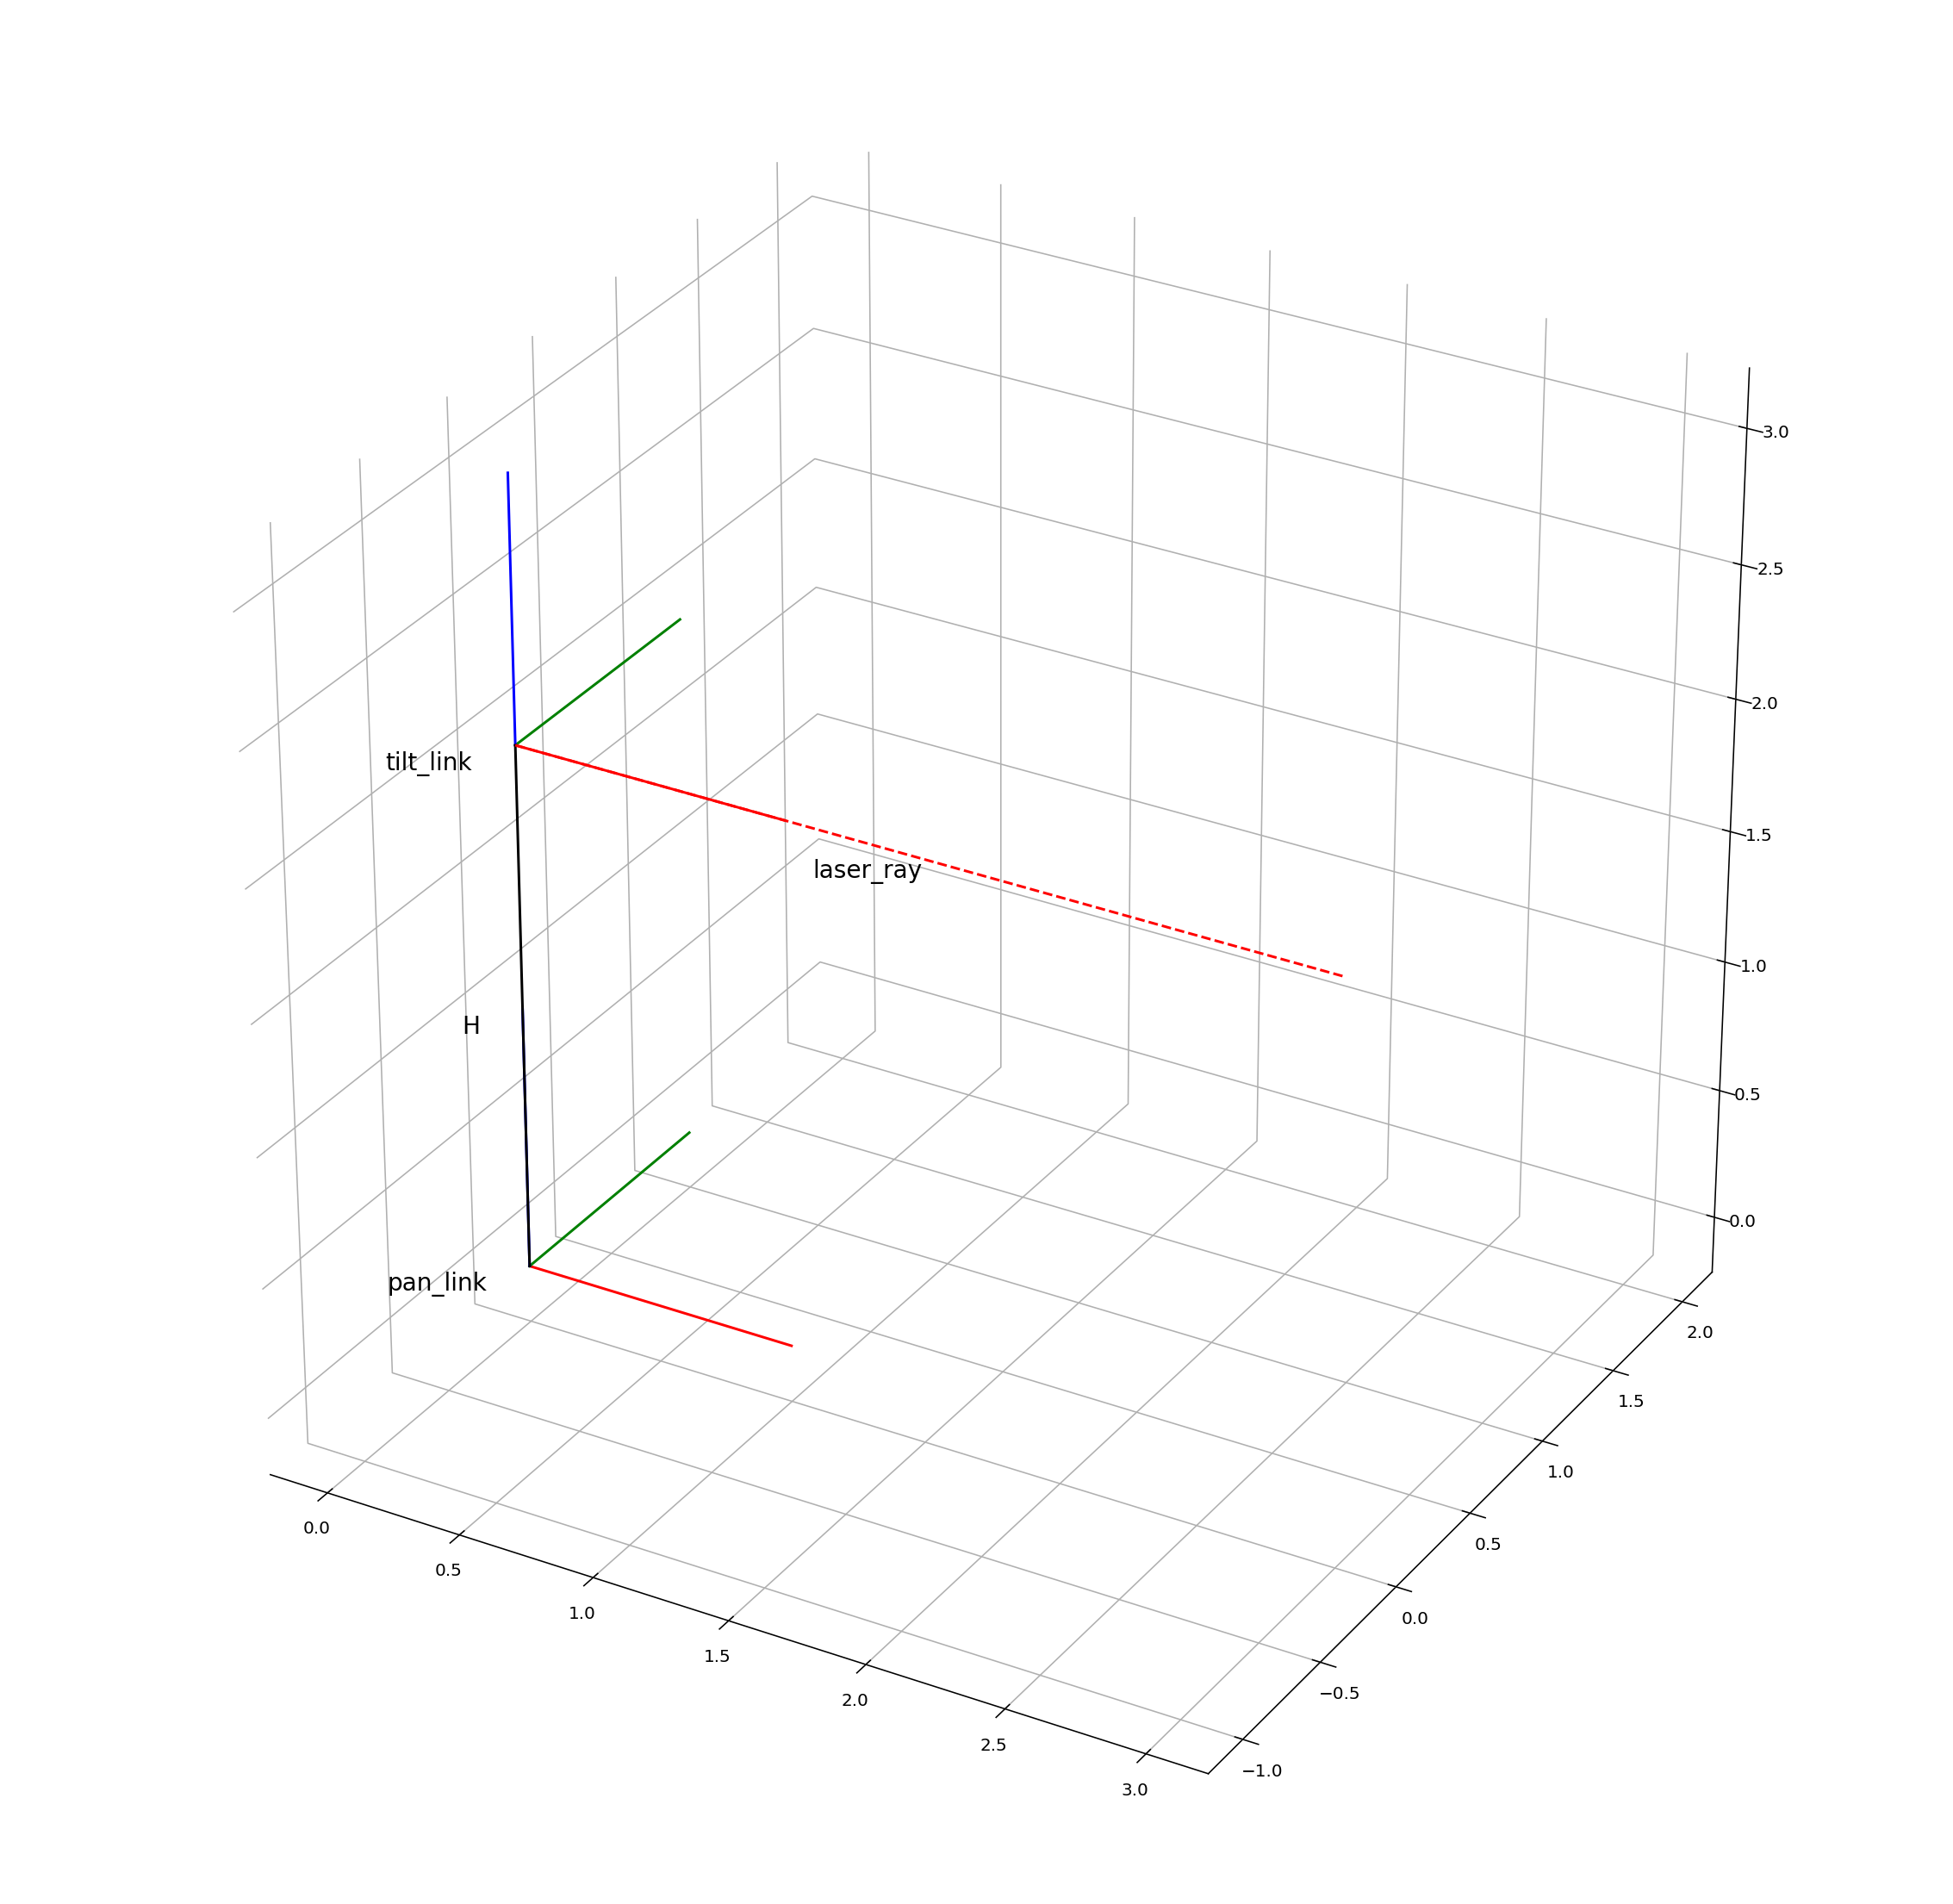
\includegraphics[width=\textwidth]{img/firstModel.png}%
	\caption{Pan and Tilt, First Model}
	\label{fig:firstModel}
\end{figure}

\\

